\documentclass[a4paper, 11pt, onepage]{scrreprt}

\usepackage{fontspec}
\setmainfont{Linux Libertine O}
\usepackage{polyglossia}
\usepackage{amssymb}
\usepackage{amsmath}
\usepackage{mathtools}
\usepackage{bbold}
\usepackage[hyperref]{xcolor}
\usepackage{graphicx}
\usepackage{listings}
\usepackage{caption}
\usepackage{wrapfig}
\usepackage{float}
\usepackage{tabularx}
\usepackage{booktabs}
\usepackage{numprint}
\usepackage{hyperref}

\newcommand\wiki{\textsc{Wikipedia}}
\newcommand\ew{\textsc{English Wikipedia}}
\newcommand\sew{\textsc{Simple English Wikipedia}}
\newcommand\tableref[1]{\hyperref[#1]{Table \ref*{#1}}}
\newcommand\figureref[1]{\hyperref[#1]{Figure \ref*{#1}}}
\newcommand\sectionref[1]{\hyperref[#1]{Section \ref*{#1}}}
\newcommand\equaref[1]{\hyperref[#1]{Equation \ref*{#1}}}
\newcommand\maps[1]{\xrightarrow{\mathcal{#1}}}
\newcommand\card[1]{\lvert #1 \rvert}
\newcommand\suchthat{\, \middle| \,}
\newcommand\given{\, \middle| \,}
\newcommand\proba[2][]{P_{#1} \left( #2 \right)}

\DeclareMathOperator*{\argmin}{\arg\,\min}
\DeclareMathOperator*{\argmax}{\arg\,\max}

\renewcommand\chaptername{Section}
\renewcommand\thechapter{\Roman{chapter}}

\DeclareGraphicsExtensions{.png, .jpeg, .jpg, .svg, .eps}
\graphicspath{{./img/}}

\hypersetup{
  colorlinks = true,
  linkcolor = violet,
  urlcolor = teal,
  citecolor = gray
}

\begin{document}
\begin{titlepage}
  \begin{center}
    \noindent\rule{\textwidth}{0.4pt}
    {\huge\bfseries Improving text readability using\\
      \sew\\}
    \noindent\rule{\textwidth}{0.4pt}\\
    % ----------------------------------------------------------------
    \vspace{1.5cm}
    {\large
    \begin{tabularx}{\textwidth}{lXll}
      \textbf{Author:} & \textsc{Hugo Mougard} &
      \textbf{Director:} & \textsc{Akiko Aizawa} \\
      \textbf{Tutor:} & \textsc{Colin de la Higuera} &
      \textbf{Advisor:} & \textsc{Pascual Martínez-Gomez} \\
    \end{tabularx}}\\[5pt]
    % ----------------------------------------------------------------
    \vfill
    \parbox{0pt}{\large \begin{tabbing}
        \textbf{Sending institution:} \= National Institute of Informatics \kill
        \textbf{Sending institution:} \> \textsc{Université de Nantes, France} \\
        \textbf{Hosting institution:} \> \textsc{National Institute of
        Informatics, Japan} \\
      \end{tabbing}}
    \vfill
    {\LARGE ATAL Master 2 internship report}
    \vfill
    % ----------------------------------------------------------------
    
\includegraphics[width=0.16\textwidth]{img/nii.png}
    \hfill
    \hfill
    
\includegraphics[width=0.19\textwidth]{img/lina.png}
    \hfill
    
\includegraphics[width=0.19\textwidth]{img/univ.eps}
    \vfill
    {July 2014}
  \end{center}
\end{titlepage}

\tableofcontents

\chapter{Acknowledgments}

I would like to thank Aizawa-sensei and Katsu-san for their precious
help before our arrival to Japan, and their support during our stay.

I also wouldn't have been able to conduct this internship without the
scientific advising of Aizawa-sensei and Pascual-san, I thank them for
all their good insight, even though I am convinced I didn't make the
best of it.

It was also very nice to have someone exterior to discuss ideas with
when I wanted to, I thank Colin de la Higuera for that.

\chapter{Laboratory presentation}

\section{\textsc{National Institute of Informatics}}
\label{sec:national-institute-of-informatics}

The \textsc{National Institute of Informatics} is a Japanese research
institute located in Chiyoda-ku, Tokyo. It has strong connections with
the \textsc{University of Tokyo} (\textsc{Todai}) and welcomes
computer scientists of numerous domains to form a strong innovative
pole in the Japanese computer science research landscape.

Its International Exchange Agreements program allowed two of the
students of the 2012−2014 promotion of the ATAL master to join for a
five month internship.

\section{\textsc{Aizawa Laboratory}}
\label{sec:aizawa-laboratory}

The team that welcomed me for this work is \textsc{Aizawa
  Laboratory}\footnote{\url{http://www-al.nii.ac.jp/en/}}. It is led
by Professor \textsc{Akiko
  Aizawa}\footnote{\url{http://research.nii.ac.jp/~akiko/index_e.html}},
the director of this internship. At the time of this writing, the
laboratory has 18 members and strong partnerships with ex-members of
the laboratory.

Its expertise lies in several sub-domains of Natural Language
Processing (NLP):
\begin{itemize}
\item NLP using gaze information;
\item analysis and mining of scientific papers;
\item mathematical information retrieval;
\item syntactic and semantic structure analysis of natural language
  text;
\item extraction and classification of technical terms.
\end{itemize}

The work presented in this report has been done in the group
interested in NLP using gaze information, mostly for historical
reasons: the work proposed during this internship doesn't use gaze
information. Still, readability — the topic of this internship — has
strong connections to gaze NLP and other members of the group were
very knowledgeable in this domain. This was a great opportunity for
the development of this internship.

\chapter{Introduction}

Whether it is to teach children how to read, to assess the
comprehensiveness of technical manuals or to better grasp how we
understand things, readability has been studied for about two
centuries for its impact in both engineering and scientific endeavors.

Despite this interest of the scientific community, an important part
of the early research has focused on finding basic metrics to measure
readability. It is only in recent years that scientists have been able
to come up with more interesting methods, thanks in particular to the
advances in machine learning, the new speed of modern computers and
the unparalleled amount of data available on the internet.

The high-level goal of this internship is to investigate those methods
and improve on them. To be more specific, most methods consider
documents as a whole when analyzing their readability, which makes it
hard for users to understand which parts are the most important to
rework. We aim at providing a fine-grained analysis of readability in
this work. In the same way than the recursive approach to sentiment
analysis \cite{socher2013recursive} allows users to detect which parts
of a sentence convey which sentiment, we aim at detecting which parts
of a sentence are readable or non readable, and for which reasons.

The approach used in this work is to combine text rewriting with
scoring techniques to achieve both readability improvement and
assessment and anchoring in the input text.

\chapter{Prior art}
\label{sec:sota}

This section details the history and state of the art of computational
readability study.

\section{Early works and readability formulas}
\label{sec:early-works-and-formulas}
Readability has been studied extensively. The first works in this area
date back to more than a century ago: in 1893, Sherman published a
book \cite{sherman1893analytics} where he compared modern English and
English spoken four centuries before with considerations that are very
alike the ones that current readability studies outline. Then, in
1921, Thorndike computed a list of ten thousand easy-to-read words
\cite{thorndike1921teacher}. This list got used shortly thereafter by
teachers trying to select good books for children learning to read
\cite{lively1923method}: they went through the process of estimating
the readability of many books thanks to a basic formula and
Thorndike's list.

This was the beginning of an important branch of research focusing on
how to best estimate the readability of a text thanks to simple
formulas. Among the most famous methods, it is interesting to mention
the Flesch Reading Ease \cite{flesch1948new} which introduced the use
of a combination of the average number of words per sentence and the
average number of syllables per word to estimate the readability of a
text. Most of the subsequent approaches also use those metrics. This
method yields a 0.91 correlation with text understanding and has been
used outside of research to improve the readability of a vast amount
of publications, yielding excellent results in readership increase.

Roughly at the same time, Dale and Chall introduced a readability
formula that uses a list a words instead of the average number of
syllables per word to estimate readability
\cite{dale1948formula}. This more precise definition of world
difficulty allows this metric to reach a 0.93 correlation with text
understanding and because of that has been one of the most used
formulas in research.

Later works brought formulas that are easier to compute or give
slightly better results. Some also give their result as the grade that
would be required to be able to read the input text. Overall are all
using the same variables as either Flesch or Dale and Chall
\cite{mclaughlin1969smog, kincaid1975derivation,
  chall1995readability}.

Despite their useful applications, readability formulas are not
perfect. Some works have detailed their problems convincingly
\cite{duffy1985readability, schriver2000readability}. Among the most
important ones is using sentence length to model syntactic complexity:
of the following sentences, (1.) is often considered easier to
understand than (2.), despite being lengthier:
\begin{enumerate}
\item The mouse ate the cheese, and then the rat ate the mouse, and
  after that, the cat ate the rat and died.
\item The cat that ate the rat that ate the mouse that ate the cheese
  died.
\end{enumerate}
Another important problem is modeling word complexity by word length,
which doesn't consider the fact that affixes are known to
readers. That makes some long words simple, while some short words
are, in contrary, relatively unknown: “curr” (to make a murmuring
sound), is for most people harder to read than reinventing, due to the
rarity of “curr” and the fact that even early readers know the meaning
of the “re-” and “-ing” affixes.

Finally, the fact that many formulas only consider short windows of a
text to estimate its readability make them not reliable without
repetition of the measure at several points in a text and an averaging
(which is what Dale \& Chall does by default).

To address those shortcomings, scientists have recently proposed
machine learning based approaches. The next section details those
works.

\section{Machine Learning approaches}
\label{sec:ml-approaches}

Readability assessment can be seen as a supervised classification
task. To predict the required grade to understand a given input text,
\cite{callanlanguage} use a unigram language model of each target
grade in order to see which one is the most likely to generate the
input.

\cite{schwarm2005reading} improve on this approach by using a trigram
model instead of a unigram model. They also incorporate classical
readability features by using a SVM with the perplexity scores of the
language models as features along with readability scores in various
formulas and syntactic features.

In 2008, Pitler and Nenkova conduct a study where they use complex
features to measure the possible improvements yet to achieve in
machine learning approached \cite{pitler2008revisiting}. Those include
discourse relations, entity coherence, syntactic and lexical
features. They notice possible improvements but conclude that until
robust automatic method to obtain those metrics exist, it is unlikely
that those improvements will be usable in a large scale system.

\section{Readability research using \wiki}
\label{sec:wiki-approaches}

From 2006 onwards, \sew has been rightly seen as an important resource
for readability studies. Scientists have used it to compute parallel
corpora of readable sentences and their hard-to-read counterparts.

\chapter{Work}
\label{cha:work}

To address the lack of corpora and tooling in the readability domain,
we propose a method to easily build a parallel corpus using \sew's
revision history. This approach is not novel, since 2008, researchers
have used \sew's revision history to great effect
\cite{nelken2008mining}. What is novel is that we plan on releasing
the corpus with a permissive license and associated tooling to reduce
the entry cost of readability research and allow comparison between
methods on a level ground.

To be able to correctly investigate fine-grained readability, we
propose a software suite to represent results of readability system in
a way that suits analysis.

Finally we experiment with lexical re-writings using our system.

Details on those three main axes follow.

A timeline of the work done finishes this introduction:

\begin{itemize}
\item March 1\textsuperscript{st} − April 1\textsuperscript{st}:
  bibliograhy;
\item April 1\textsuperscript{st} − April 8\textsuperscript{th}:
  subject design;
\item April 8\textsuperscript{th} − May 8\textsuperscript{th}:
  parallel corpus creation;
\item May 8\textsuperscript{th} − June 18\textsuperscript{th}:
  joint work on the demo and the scoring methods, with explorations of
  other methods;
\item June 18\textsuperscript{th} − July 10\textsuperscript{th}:
  report and internship defence preparation.
\end{itemize}

\section{Automatic readability parallel corpus creation}
\label{sec:corpus}

Machine learning approaches are used more and more and in a wide range
of scientific domains for their effectiveness. Most of the time, the
more data you have, the best your results will be, up to an extent
that people to described data efficiency as “unreasonable”
\cite{halevy2009unreasonable}. In this context, it seems that being
able to gather automatically data is of utmost importance. Moreover,
raw data is often not enough. Most techniques require a lengthy and
costly annotation process. For this reason, researchers in every
domain using machine learning invest time finding clever techniques to
automatically obtain annotated corpora.

In readability, such a clever technique is to leverage the power of
\wiki, and in particular \sew. To do so, mainly two techniques have
been used: the first is to align the articles present both in the
regular \ew{} and in \sew{} to build a parallel corpus. This approach
has been used with great success in
\cite{zhu-bernhard-gurevych:2010:PAPERS} and has resulted in the
PWKP-108016\footnote{\url{https://www.ukp.tu-darmstadt.de/data/sentence-simplification/simple-complex-sentence-pairs/}}
dataset. The second is to use the revision history of \sew, as
showcased in \cite{yatskar2010sake}. In this work we use the second
approach.

The main rationale behind not using the existing PWKP-108016 corpus
and instead creating one of our own is that we believe the technique
used to automatically construct the corpus from a revision history is
a general process and can therefore be extended to many data sources
beyond \wiki. Those possible extensions include many of the processes
of the professional publishing world. If proven efficient, big corpora
could be gathered from journalists, writers, scientists, etc. On the
contrary, it has been shown to be extremely hard to find good
comparable corpora outside of \wiki{} and some restricted institution
publications such as the European Parliament \cite{koehn2005europarl},
which makes the first approach hard to generalize. Finally, the
outputs made public by \cite{yatskar2010sake} are of high quality but
limited in quantity and do not incorporate some important features
such that the original sentence from which pairs were extracted, nor
does this release include any code to manipulate the files.

To build automatically our corpus, we leverage the fact that when
editing \sew, contributors have the possibility to write a commit
message, so that other people can quickly browse history and guess the
role of a particular commit. This allows us to automatically detect if
a particular commit was intended to fix a readability issue or was
serving another purpose (improving the content of the article,
cleaning the wiki, vandalizing, …). This usage of metadata is not
novel, it was used in the \textsc{Simpl} approach presented in
\cite{yatskar2010sake}. Though, we fine-tune the heuristic used to
address some problems encountered in this article and to harden the
process. An example of readability edit can be seen in
\figureref{fig:dan-kelly}.

\begin{figure}[H]
  \centering
  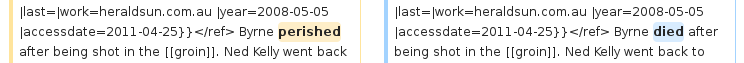
\includegraphics[width=\textwidth]{dan-kelly}
  \caption{An edit of the Dan Kelly article with the commit message
    “use simple english here”}
  \label{fig:dan-kelly}
\end{figure}

The heuristic we use to gather edits is extremely simple: once
stripped of the category information, we only consider edits with
commit messages $m$ so that:

\[
m \in \left\{\text{“simplify”}, \text{“simplifying”},
  \text{“simplified”}, \text{“simplification”},
  \text{“simpler”}\right\}
\]

This may seem drastic but we believe it is necessary due to the many
noisy commits introduced with broader rules. To illustrate this point,
we can consider the commit messages of
\tableref{tab:problematic-commits}. We can see that commit \#1 has two
purposes, one of which will bring noise (the wikification). Commit \#2
contains one of the matching terms, but we should not consider
it. It's not clear if commit \#3 tries to address readability or not.

\begin{table}[H]
  \centering
  \caption{Problematic commit messages}
  \begin{tabular}{rp{12cm}}
    \toprule
    \# & Commit message \\
    \midrule
    1 & “simplified, and wikified” \\
    \addlinespace
    2 & “wikify. needs simplifying” \\
    \addlinespace
    3 & “exhaustive, to help us work out titles of articles - lots of
    discussion here, and no, this is not simple engouh yet” \\
  \end{tabular}
  \label{tab:problematic-commits}
\end{table}

Furthermore, we determined by an empirical study that those commits
represented an important part of the commits we might have retrieved
with a broader rule, so we simply did not consider them.

The next step for the creation of the corpus is to compute the precise
edit that the contributor made. To do so, we tokenize and sentence
split both the original version of the article and its revision using
OpenNLP\footnote{\url{https://opennlp.apache.org/}}. Then, we use
Myers' alignment algorithm \cite{myers1988optimal} to compute optimal
alignments at the world and sentence levels. We rely on the
implementation proposed by
jgit\footnote{\url{http://www.eclipse.org/jgit/}}.

The goal being to obtain a re-usable corpus, we propose the complete
pipeline on
github\footnote{\url{https://github.com/m09/readability}}. It is
freely re-usable.

The obtained corpus has important noise problems. A quick glance at
\tableref{tab:problematic-edits} is sufficient to understand that some
edits are not readability edits, but either alignment deficiencies or
edits serving complementary roles. When filtered to only consider
revisions of 5 words at most, to match the policy used in
\cite{yatskar2010sake}, the number of entries is reduced to
\numprint{23507}.

\begin{table}[H]
  \centering
  \caption{Problematic edits}
  \begin{tabular}{rp{6cm}p{6cm}}
    \toprule
    \# & Original version & Revised version \\
    \midrule
    1 & , and & . she also used them in her arguments about \\
    \addlinespace
    2 & 2010 federal election, is russell matheson, a member & size\\
  \end{tabular}
  \label{tab:problematic-edits}
\end{table}

The unfiltered corpus has \numprint{43753} entries. However, it has
important noise problems. A quick glance at
\tableref{tab:problematic-edits} is sufficient to understand that some
edits are not readability edits, but either alignment deficiencies or
edits serving complementary roles. When filtered to only consider
revisions of 5 words at most, to match the policy used in
\cite{yatskar2010sake}, the number of entries is reduced to
\numprint{23507}.  The resulting resource is enriched with
part-of-speech, and syntactic parsing annotations and is proposed in
an XML format to optimize re-usability.

\section{Lexical enhancements}
\label{sec:lexical-enhancements}

With this corpus at our disposal, we next define a way to use it as a
lexical dictionary. The goal is to allow authors to pick simpler words
than the ones they used, in an efficient manner. In what follows, we
will denote multiset of all rewritings of $x$ in $y$ in $\mathcal{D}$
by $x \maps{D} y$ a,d we will use $\_$ as a wildcard to denote any
word.

The first approach and the most basic one, given a dictionary
$\mathcal{D}$ and for a word $w$, is to propose as lexical rewriting
candidates the set $R_w$ such that:

\[
R_w = \left\{r \suchthat w \maps{D} r\right\}
\]

But obviously, while this approach will have a important recall, it
will be extremely noisy and will not be of any real help to an author,
the time lost cruising through the noise outweighing the benefits of
the correct lexical enhancements.

A first improvement is to use the part of speeches available in the
corpus to make sure they match. That will already somewhat reduce
lexical ambiguity. That allows us to refine the definition of $R_w$ as
follows, $p_w$ being the part of speech of $w$:

\begin{equation*}
  R_w = \left\{
    r \suchthat u \maps{D} r \land u = w \land p_u = p_w
  \right\}
\end{equation*}

This is not enough. It would be practical to be able to compare
rewritings and rank them from the worst to the best. Rewriting scoring
functions are introduced to achieve that.

Maybe the most obvious scoring function is one that gives a score to a
rewriting that reflects how often it occurs in the corpus
$\mathcal{D}$. The probability $\proba{w \maps{D} r}$ of a rewriting
from $w$ to $r$ occurring in $\mathcal{D}$ is computed as follows:

\begin{equation*}
  \proba{w \maps{D} r} = \frac{\card{w \maps{D} r}}{\card{\_ \maps{D} \_}}
\end{equation*}

\equaref{eq:socc} expresses the score function $\mathcal{S}_{OCC}$
that uses this probability and measures how often a rewriting occurs.

\begin{equation}
  \label{eq:socc}
  \mathcal{S}_{OCC}(w \maps{D} r) = \log \proba{w \maps{D} r}
\end{equation}

We take the log to ensure the numerical precision of the computations
despite the imprecision of floating point arithmetic for small values.

Even though this score is a great starting point, it is not a good
score to evaluate lexical rewritings. Its main shortcoming is that it
outlines mainly punctuation and non-content words rewritings. Those
are mainly linked to syntax and cannot be handled by a purely lexical
rewriting system at any acceptable level of performance. The following
scores try to fix this punctuation and non-content words focus to turn
it into a lexical focus.

To accomplish this shift, we define the quality of a rewriting of $w$
into $r$ as the probability of a human rewriting $w$ into $r$. By
combining a language model to the information present in the corpus
$\mathcal{D}$, it is possible to derive a measure close to this
probability.

The score $\mathcal{S}_{LM}$ is one way to capture the above
definition, with $\proba[LM]{w}$ the language model probability of
$w$:

\begin{align}
  \label{eq:slm1}
  \mathcal{S}_{LM}(w \maps{D} r) & = \log \frac{\proba{w \maps{D} r}^\lambda}%
  {\proba[LM]{w}^{(1 - \lambda)}} \\
  \label{eq:slm2}
  & = \lambda \mathcal{S}_{OCC} - (1 - \lambda) \log \proba[LM]{w}
\end{align}

The two equations above explain $\mathcal{S}_{LM}$ in two different
ways. \equaref{eq:slm1} best shows that $\mathcal{S}_{LM}$ is an
approximation of the ratio of the number of times a word is rewritten
on the number of times it appears. \equaref{eq:slm2} best shows that
$\mathcal{S}_{LM}$ is a balancing act: both $\mathcal{S}_{OCC}$ and
$\log \proba[lm]{w}$ are negative quantities: by subtracting one to
the other we balance two properties of a good rewriting. $\lambda \in
\left[0,1\right]$ is a parameter to control this balancing.

Another take on this problem is to consider that good lexical
rewritings are good rewritings of rarely occurring words. This
definition is well captured by the conditional probability defined in
\equaref{eq:probcond} and its application to the score
$\mathcal{S}_{LMc}$ defined in \equaref{eq:slmc}. $c$ stands for
“conditional”:

\begin{align}
  \label{eq:probcond}
  \proba{w \maps{D} r \given w \maps{D} \_} & = \frac%
  {\card{w \maps{D} r}}%
  {\card{w \maps{D} \_}} \\
  \label{eq:slmc}
  \mathcal{S}_{LMc}(w \maps{D} r) & = \log \frac%
  {\proba{w \maps{D} r \given w \maps{D} \_}^\lambda}%
  {\proba[lm]{w}^{(1 - \lambda)}}
\end{align}

The scores $\mathcal{S}_{LM}$ and $\mathcal{S}_{LMc}$ already have
nice qualities to model different definitions of good rewritings. But
as they stand, the lengthier the word being rewritten, the better the
score of its rewriting, almost regardless of whether or not the
rewriting is a good lexical rewriting or not. This happens because the
language model probability of a $(n+1)$-gram is almost always an order
of magnitude lower than the language model probability of a
$n$-gram.

Concretely it means that the rewriting of a bigram such as “\emph{,
  and} $\rightarrow$ \emph{.}”  will come above most lexical
rewritings, such as the rewriting “\emph{exhausted} $\rightarrow$
\emph{tired}”. Taking into account the length of the sequence being
rewritten allows to fix that. The scoring functions
$\mathcal{S}_{LMw}$ and $\mathcal{S}_{LMcw}$ are extensions of
respectively the scoring functions $\mathcal{S}_{LM}$ and
$\mathcal{S}_{LMc}$ and are introduced to average the language model
scores by considering the length of the words considered. $w$ stands
for “weighted”:

\begin{align}
  \label{eq:slmw}
  \mathcal{S}_{LMw}(w \maps{D} r) = & \log \frac%
  {\proba{w \maps{D} r}^\lambda}%
  {\sqrt[\card{w}]{\proba[lm]{w}}^{(1 - \lambda)}} \\
  \label{eq:slmcw}
  \mathcal{S}_{LMcw}(w \maps{D} r) = & \log \frac%
  {\proba{w \maps{D} r \given w \maps{D} \_}^\lambda}%
  {\sqrt[\card{w}]{\proba[lm]{w}}^{(1 - \lambda)}} \\
\end{align}

The method used in both \equaref{eq:slmw} and \equaref{eq:slmcw} to
weight a language model score by its length $l$ is to take its
$l^{th}$-root. This is justified by the fact that language model
scores follow a power law when subjected to the length of their input
sequences.

Note that while we progressively improved the lexical properties of
the scoring functions over the course of this section, the results of
those functions are not the log of probabilities anymore, which is not
a problem to compare rewritings but might very well be to use those
rewriting scores in a broader framework, for example when performing
the automatic rewriting of a text. We deal with this task — and those
issues — in the next section.

\section{Automatic rewriting of texts}
\label{sec:rewriting}

% expliquer why transducers et semi-anneau

To rewrite texts automatically, we use weighted finite-state
transducers that consider the scores defined
in \sectionref{sec:lexical-enhancements} as weights to rewrite any
input text. By doing so we consider the rewriting of texts as a
translation task from the language of hardly readable texts to the
language of readable texts.

Two of the main tasks performed while manipulating weighted
transducers are combining weights in a given branch and combining the
weights of two different branches. Those two operations require
respectively a product and a sum and therefore semi-rings are commonly
used to model the way weights are handled in a weighted transducer
\cite{mohri2004weighted}.

We define a weighted finite-state transducer over a semi-ring
$(\mathbb{K}, \oplus, \otimes, \mathbb{0}, \mathbb{1})$ (that we will
use to combine the outputs of a score function) as an 8-tuple that
follows the common definition used by \cite{mohri2004weighted}: $T =
(\Sigma, \Delta, Q, I, F, E, \lambda, \rho)$ where:
\begin{itemize}
\item $\Sigma$ is the finite input alphabet of the transducer;
\item $\Delta$ is the finite output alphabet;
\item $Q$ is a finite set of states;
\item $I \subseteq Q$ the set of initial states;
\item $F \subseteq Q$ the set of final states;
\item $E \subseteq Q \times (\Sigma \cup \{\varepsilon\}) \times
  (\Delta \cup \{\varepsilon\}) \times \mathbb{K} \times Q$ a finite
  set of transitions;
\item $λ : I \rightarrow \mathbb{K}$ the initial weight function;
\item $ρ : F \rightarrow \mathbb{K}$ the final weight function mapping
  $F$ to $\mathbb{K}$.
\end{itemize}
Such a transducer over a semi-ring $(\mathbb{K}, \oplus, \otimes,
\mathbb{0}, \mathbb{1})$ is constructed for a given input text of $n$
tokens noted $t_1 \dots t_n$ and their $n$ parts of speech noted $p_1
\dots p_n$ as follows, where $\mathcal{T}$ is the set of all tokens in
written English, $\mathcal{P}$ is the set of all parts of speech in
English and $\mathcal{S} : \mathcal{D} \rightarrow \mathbb{K}$ is the
score we use, $\mathbb{K}$ being the set of the semi-ring:
\begin{itemize}
\item $\Sigma = \mathcal{T} \times \mathcal{P}$;
\item $\Delta = \mathcal{T} \times \mathcal{P}$;
\item $Q = \left\{ q_i \suchthat 0 \leq i \leq n \right\}$;
\item $I = \{ q_0 \}$;
\item $F = \{ q_n \}$;
\item $E = \left\{ (q_{i - 1}, w, r, s, q_i) \suchthat w \maps{D} r
    \land w = t_i \land p_w = p_i \land s = \mathcal{S}\left(\ t_i
      \maps{D} r \right)\right\}$;
\item $I : x \mapsto \mathbb{1}$;
\item $F : x \mapsto \mathbb{1}$.
\end{itemize}
Now, we can define semi-rings to use with the constructed
transducer. We mainly consider two use-cases, each of them requiring a
different semi-ring:

\begin{figure}[H]
  \centering
  \begin{enumerate}
  \item from the transducer and an input text, calculate the top $n$
    transductions. This is the classical of statistical machine
    translation;
  \item from the transducer and an input text, get an idea of how the
    system rewrites the text at a certain level of confidence.
  \end{enumerate}
  
  \caption{Use-cases of text rewriting}
\label{fig:use-cases}
\end{figure}

The motivation for the second use-case is maybe not clear at
first. The reason for its existence is that, even for a very long
text, a top 100 of the rewritings might very well return 100 different
single token modifications while we would want to see the complete
text rewritten at once at a certain level of confidence.

We define the semi-rings in \tableref{tab:semi-rings} for the
$S_{OCC}$ score function. The Negative MaxMin semi-ring allows us to
obtain the threshold effect of use-case (2.) from
\figureref{fig:use-cases} while the Negative Log semi-ring allows us
to compute the precise tops of use-case (1.). Negative Log is the log
equivalent of the $(\left[0, 1\right], +, *, 0, 1)$ semi-ring for
probabilities.

\begin{table}[H]
  \centering
  \begin{tabular}{rccccc}
    \toprule
    Semiring & $\mathbb{K}$ & $\oplus$ & $\otimes$ & $\mathbb{0}$ & $\mathbb{1}$
    \\
    \midrule
    Negative Log & $\mathbb{R}^{-} \cup \{-\infty\}$ & $+_{\log}$ & $+$ & $-\infty$ & $0$ \\
    Negative MaxMin & $\mathbb{R}^{-} \cup \{-\infty\}$ & $\max$ & $\min$ & $-\infty$ & $0$ \\
  \end{tabular}
  \caption{Interesting semi-rings for our score functions, where
    $a +_{\log} b = \log\left(e^a + e^b\right)$}
  \label{tab:semi-rings}
\end{table}

Those semi-rings are almost usable with the various flavors of
$\mathcal{S}_{LM}$ score functions. But since they are not the log of
probabilities, we don't have the guarantee that for all $w \maps{D}
r$, $\mathcal{S} \left( w \maps{D} r \right) \in \left]-\infty,
  0\right]$. To fix this problem, we normalize the scores
$\mathcal{S}_{LM}$ and $\mathcal{S}_{LMc}$ into the scores
$\mathcal{S}_{LMn}, \mathcal{S}_{LMcn}$ as follows ($n$ standing for
normalized):

\[
\mathcal{S}_{n} \left( w \maps{D} r \right) = \mathcal{S} \left( w
  \maps{D} r \right) + \argmin_{w'} \left( \log \proba[lm]{w'} \right)
\]

And the scores $\mathcal{S}_{LMw}$ and $\mathcal{S}_{LMcw}$ into the
scores $\mathcal{S}_{LMwn}, \mathcal{S}_{LMcwn}$ as follows:

\[
\mathcal{S}_{n} \left( w \maps{D} r \right) = \mathcal{S} \left( w
  \maps{D} r \right) + \argmin_{w'} \left( \log
  \sqrt[\card{w'}]{\proba[lm]{w'}} \right)
\]

The normalized functions can be used with the semi-rings we defined
for $\mathcal{S}_{OCC}$.

It is now possible to address the two use-cases mentioned in
\figureref{fig:use-cases} by using the Viterbi algorithm
\cite{forney1973viterbi} with Negative Log as semi-ring for the first
use-case and Negative MaxMin for the second.

The next section details \textsc{Readability Lab}, a framework built
to analyze both lexical enhancements and text rewritings in an
intuitive and efficient manner.

\section{\textsc{Readability Lab}, a fine-grained readability analysis
  framework}
\label{sec:framework}

Considering that automatic evaluation of readability rewriting and
lexical enhancement is a very hard task, producing a high quality
testing environment to be able to quickly assess manually the quality
of an approach is valuable. It was also the occasion to expose those
results to other programs by creating a server that could easily be
used by from other tool-chain.

\href{http://www.playframework.com/}{Play Framework} and
\href{https://facebook.github.io/react/}{React} were used to create a
web client that satisfies the constraints exposed
above. \figureref{fig:ui} shows a screenshot of the interface.

Among the challenges faced during the creation of this demo, the most
interesting one is certainly the algorithm used to detect matches in a
text. Indeed, with more than \numprint{20000} patterns to test,
response times easily grow slow. To address this issue, we used the
Aho-Corasick algorithm \cite{aho1975efficient} on the alphabet of
pairs of a token and its part of speech. The principle of this
algorithm is to build an automaton to match patterns that is
afterwards usable on any incoming text.

This matches perfectly the structure of a web application where this
automaton can be built once, slowly, and then used to provide
extremely fast search on incoming requests for all the lifetime of the
server. Since no existing implementation that we knew of had
abstracted away the alphabet used, a new implementation has been
proposed that addresses this issue and allows to use arbitrary Java
classes as alphabet (here our pairs of token and their part of
speech).

\begin{figure}[H]
  \centering
  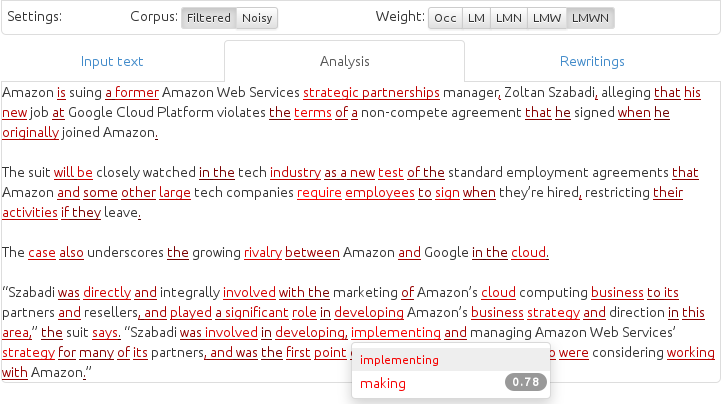
\includegraphics[width=\textwidth]{ui}
  \caption{\textsc{Readability Lab} interface}
  \label{fig:ui}
\end{figure}

\chapter{Open source contributions}
\label{cha:oss-contribs}

During this internship I had the opportunity to contribute to the open
source natural language processing community. What follows is a list
of those contributions.

\section{Enhancements of existing software}
\label{sec:enhancements}

\begin{itemize}
\item
  \href{https://bugs.eclipse.org/bugs/show_bug.cgi?id=433163}{Wikitext
    parser bug filing}
\item \href{https://issues.apache.org/jira/browse/OPENNLP-676}{OpenNLP
    POSTagger bug filing with patch}
\item \href{https://issues.apache.org/jira/browse/UIMA-3913}{uimaFIT
    enhancement proposal}
\end{itemize}

\section{\textsc{uimaFIT} components}
\label{sec:uimafit-components}

\begin{itemize}
\item sentence alignment analysis engine, using Myers' algorithm
\item word alignment analysis engine, using yet again Myers' algorithm
\item \href{https://berkeleylm.googlecode.com/}{BerkeleyLM} uimaFIT
  wrapper
\item readability formulas uimaFIT calculator
\end{itemize}

\section{Miscellaneous}
\label{sec:misc-software}
\begin{itemize}
\item Wikimedia PostgreSQL importer
\item Generic implementation of Aho-Corasick
\end{itemize}

\chapter{Conclusions  et perspectives}

\bibliographystyle{apalike2}
\bibliography{report.bib}

\end{document}
%%% Local Variables: 
%%% coding: utf-8
%%% mode: latex
%%% TeX-engine: xetex
%%% End: 
